\chapter{Theoretical Background}

In the following sections, the theoretical foundations of every major concept behind the experimental phase of the assignment will be discussed.

\section{Discriminative and Generative Models}

\textit{Discriminative} and \textit{Generative} are two classes of machine learning algorithms, each with quite different characteristics from the other.

\paragraph{Generative} Generative models are models where the focus is the distribution of individual classes in a dataset and the learning algorithms tend to \textit{model the underlying patterns/distribution of the data points}. These models use the intuition of joint probability in theory, creating instances where a given feature $x$ (input) and the desired label $y$ (output) exist at the same time.
Generative models use probability estimates and likelihood to model data points and distinguish between different class labels in a dataset. These models are capable of generating new data instances. However, they also have a major drawback: they are incapable of effectively dealing with outliers and hence significantly affected by them.

\paragraph{Discriminative} Discriminative models tend to learn the boundary between classes/labels in a dataset. Unlike generative models, the goal here is to \textit{find the decision boundary separating one class from another}.
So while a generative model will tend to model the joint probability of data points and is capable of creating new instances using probability estimates and maximum likelihood, discriminative models (just as in the literal meaning) separate classes by rather modeling the conditional probability and do not make any assumptions about the data point. They are also not capable of generating new data instances.
Discriminative models have the advantage of being more robust to outliers, unlike the generative models.
\newline
\par
In other words, \textbf{discriminative algorithms focus on how to distinguish cases}. Hence, they focus on learning a decision boundary. On the other hand, \textbf{generative algorithms learn the fundamental properties of the data} and how to generate it from scratch.

\begin{figure}[h]
    \centering
    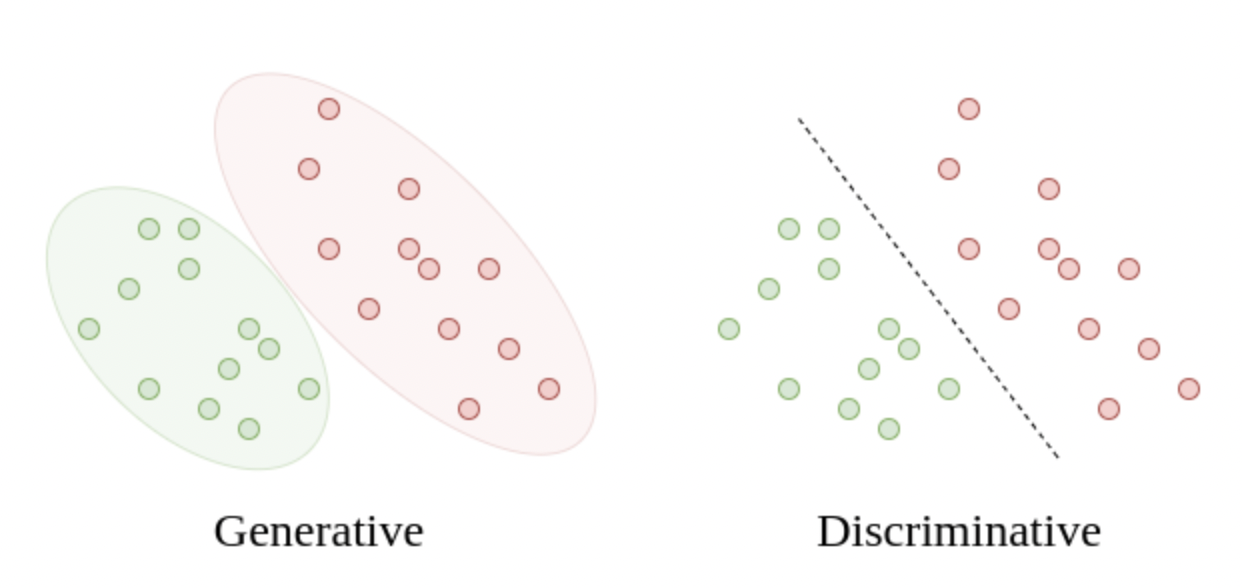
\includegraphics[scale=0.75]{images/gen-discr-models/gen-vs-discr-visual.png}
    \caption{Discriminative models try to draw boundaries in the data space, while generative models try to model how data is placed throughout the space.}
    \label{fig:gen_vs_discr_visual}
\end{figure}

\subsection{Some Examples}

Let's now look at some examples to better grasp the focus and behavior of generative and discriminative algorithms.

\paragraph{Example 1} Let’s assume our task is to determine the language of a text document. How do we solve this task with the help of machine learning?

\begin{itemize}
    \item We can learn each language and then determine the language. This is how generative models work.

    \item Alternatively, we can learn just the linguistic differences and common patterns of languages without actually learning the language. This is the discriminative approach. In this case, we don’t speak any language.
\end{itemize}

\paragraph{Example 2} Let's assume our task is to recognize images of boats.

\begin{itemize}
    \item A generative model for images might capture correlations like "things that look like boats are probably going to appear near things that look like water" and "eyes are unlikely to appear on foreheads".

    \item In contrast, a discriminative model might learn the difference between "sailboat" or "not sailboat" by just looking for a few tell-tale patterns. \textit{It could ignore many of the correlations that the generative model must get right}.
\end{itemize}


\break
\section{Support Vector Machines}

Support Vector Machine is a discriminative machine learning model whose goal is to find, through a geometrical approach, the best separating hyperplane for a dataset of points belonging to two different classes. This algorithm, given some point to make a prediction for, outputs the distance of that point from the separating hyperplane, and the sign of such a distance determines the predicted class for the input.
SVMs are based on the so called \textit{support vectors}, which are the points belonging to different classes that are the closest to each other. The position of the support vectors with respect to the separating hyperplane determines the \textit{margin}, which is a sum of distances that must be maximized in order to find the optimum decision boundary. 
Below a visual representation of the aforementioned geometrical concepts is given.

\begin{figure}[h]
    \centering
    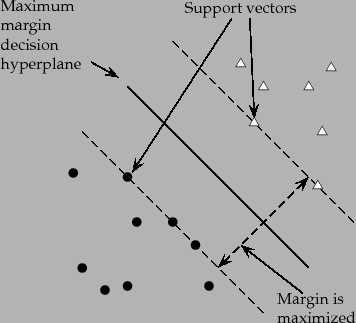
\includegraphics[scale=0.75]{images/svm/margin-support-vectors-visual.png}
    \caption{It is noted that the margin is the sum of the distances of two opposing support vectors from the separating hyperplane}
    \label{fig:svm_geom_concepts_visual}
\end{figure}

\subsection{Hard and Soft Margin}

What happens, however, if there are outliers in the training set that affect how the separating hyperplane is determined? A hardness coefficient, usually referred to as $C$, can be introduced, with the purpose of assigning a weight to misclassification errors. Its intuitive meaning is that if $C$ is high, the separating hyperplane will be calculated by trying to avoid misclassifications as much as possible, with the cost of having a reduced margin; conversely, if $C$ low, the algorithm will give more importance in finding a hyperplane with a wide enough margin. As an example, the below image allows to visualize the meaning of the $C$ parameter.

\begin{figure}[h]
    \centering
    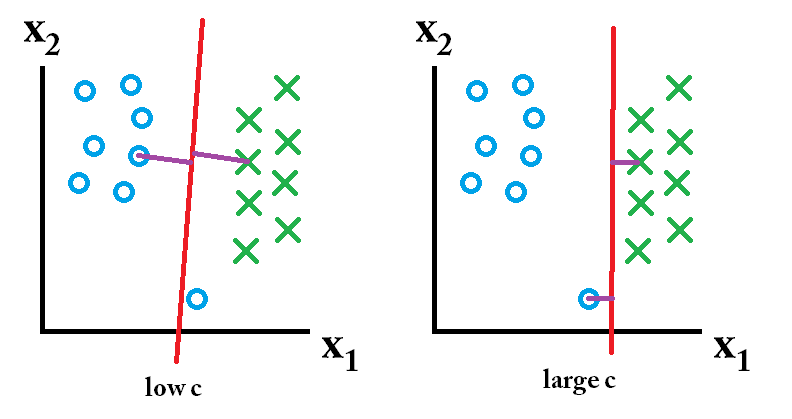
\includegraphics[scale=0.75]{images/svm/hardness-vs-softness.png}
    \caption{It is noted how there is a clear tradeoff between allowing misclassification errors and finding a separating hyperplane with a wide margin}
    \label{fig:svm_hard_soft_margin}
\end{figure}

With a low error tollerance, that is, a high value of $C$, the margin is referred to as \textbf{hard}. Viceversa, a low value of $C$ highlights a \textbf{soft} margin.


\subsection{Kernel Trick and Complexity}\label{svm_kernel_trick_and_complexity}

As previously mentioned, margin hardness determines the tolerance to misclassification errors, and tuning it is one of the approaches used to solve the problem of non-linearly separable data, that is, data for which a perfectly separating hyperplane cannot be found. Another method to consider is that of applying a higher dimensional transformation to the feature space through the so called \textit{kernel}: the same problem projected into higher dimensions is potentially linearly separable.

\begin{figure}[h]
    \centering
    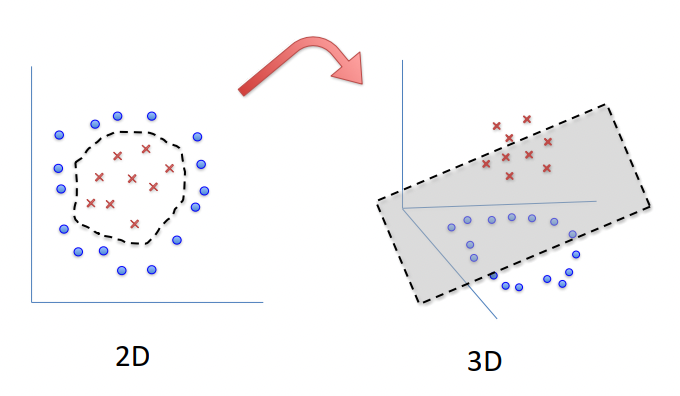
\includegraphics[scale=0.75]{images/svm/higher-dim-transform.png}
    \caption{On the left is a collection of points that isn't linearly separable. By projecting such data into three dimensions, however, a separating hyperplane can be found.}
    \label{fig:svm_higher_dim_transform}
\end{figure}

\paragraph{What is a Kernel?} A \textit{kernel} is a function $K(x, y)$ that allows to obtain the scalar product between two vectors $x, y$ in the new feature space. In particular, let $\phi(\cdot)$ be the feature space transformation function, then the kernel function is such that $K(x, y) = \phi(x) \cdot \phi(y)$.

\paragraph{Kernel Trick} It then seems that in order to train a support vector machine and optimize our objective function, we would have to perform operations with the higher dimensional vectors in the transformed feature space. In real applications, there might be many features in the data and applying transformations that involve many polynomial combinations of these features will lead to extremely high and impractical computational costs.
The kernel trick provides a solution to this problem. The \textit{“trick”} is that the kernel function acts as a modified dot product that accepts inputs in the original lower dimensional space and returns the dot product of the transformed vectors in the higher dimensional space. This means that explicitly applying the transformations $\phi(x)$ and representing the data by these transformed coordinates in the higher dimensional feature space, which is computationally expensive, can be avoided.

\paragraph{A Note on Complexity} In kernel methods, the dataset $X$ is represented by an $n \times n$ kernel matrix of pairwise similarity comparisons where the entries $(i, j)$ are defined by the kernel function $K(x_i, x_j)$. This is notable because it entails high space and computational requirements. In particular, there is theoretical and empirical evidence that, in common implementations, space complexity is $O(n^2)$ and time complexity is $O(n^3)$, the latter due to the need of computing the inverse of the kernel matrix in order to solve the underlying optimization problem \cite{SVM_Complexity}. 

\paragraph{Notable Kernels} Below follows a list of notable kernel functions. In particular, these are the ones that this assignment requires to test: 

\begin{itemize}
    \item \textbf{Linear Kernel}: $K(x_i, x_j) = x_i \cdot x_j$

    \item \textbf{Polynomial Kernel, 2nd Degree}: $K(x_i, x_j) = (1 + x_i \cdot x_j)^2$

    \item \textbf{Radial Basis Function (RBF) Kernel}: $K(x_i, x_j) = \exp{(-\frac{1}{2} \frac{(\lVert x_i - x_j \rVert)^2}{\sigma^2})}$
\end{itemize}


\break
\section{Random Forests}

The Random Forest is a discriminative machine learning algorithm that consists of applying the \textit{bagging} technique to \textit{decision trees}. Before further explaining the characteristics of random forests, the aforementioned concepts of bagging and decision trees will be introduced in the following subsections.

\subsection{Decision Trees}

The Decision Tree is a discriminative machine learning algorithm based around the concepts of predicates and splits.
In a decision tree, each node is associated to a predicate, which defines how the data is split and, consequently, how it \textit{"traverses"} the tree, and a class, in the case of the classification problem, which is determined through the process of majority voting. The final decisions of the tree are determined by the leaves and the class associated to them.

\subsubsection{Example Decision Tree Algorithm}

The algorithm to build a decision tree is, as previously mentioned, based on the concepts of split and predicate and, in particular, the goal is to determine in which way the data is best divided. Another important concept to be introduced is the concept of \textit{split gain}, which is defined as follows:

$$
Gain(split\ predicate, D) = Cost(D) - \left(\frac{\mid D_1 \mid}{\mid D \mid} \cdot Cost(D_1) + \dots + \frac{\mid D_n \mid}{\mid D \mid} \cdot Cost(D_n)\right)
$$

where $D_1 \dots D_n$ are the dataset partitions resulting from the split of $D$ and $Cost(D_k)$ is a measure of cost assgined to $D_k$, which can vary in meaning, from misclassification error to some form of disorder of the data. The intuitive meaning behind the above mathematical definition is that the best split is the one that improves the cost of the dataset pre-split $D$ the most; if such a gain is $0$, then the node at which the split is applied becomes a leaf. It is noted that the gain is always non-negative.
Below is an example recursive algorithm, written in pseudocode, that helps understand, albeit at a high level, how a decision tree is made and what it consists of.

\begin{breakablealgorithm}
	\caption{Decision Tree Algorithm} 
	\begin{algorithmic}[1]
		\Statex \textbf{Input:} Current node $N$, Dataset $D$ at the node $N$

        \State For each feature $f$ of $D$ and for each threshold $t$ of $f$ (where thresholds are all the possible values that $f$ can take): find the binary predicate $best\_split = (f \leq t)$ that achieves the highest split gain

        \State If $best\_split = 0$, then $N$ is a leaf, whose associated class is the one which is the most frequent in $D$. The algorithm stops and doesn't return anything.

        \State Create a new node $X$ associated to the predicate $best\_split$, which splits the data into two new $D_{right}, D_{left}$ partitions

        \State Recursively build the right and left subtrees using $X$ and $D_{right}, D_{left}$

        \State Return the new node $X$
		
		\item[] % newline

	\end{algorithmic}\label{alg:raptor}
\end{breakablealgorithm}

The previously mentioned $Cost$ measure is usually implemented as the degree of disorder in the dataset (partition) at the node that is being examined. In this regard, the two most common approaches are the \textit{Information Gain} and \textit{Gini Index}.

\paragraph{Information Gain} Based around the concept of entropy, the information gain is defined as the reduction in entropy that a split achieves over the pre-split dataset.
In particular, when referring to the previosuly highlighted $Gain$ and $Cost$ definitions:

$$
Cost(D) = Entropy(D) = -\sum_{i=1}^{m}{p_i \log_2{(p_i)}}
$$

It is noted that $Entropy(D)$ is maximum ($\log_2{m}$)when the $m$ classes are equally distributed in $D$ and it is minimum ($0$) when $D$ contains only one class

\paragraph{Gini Index} Like Information Gain, it favours \text{"pure"} partitions, that is, datasets containing only one class. The \textit{Gini} cost measure is defined as follows:

$$
Cost(D) = Gini(D) = 1 - \sum_{i=1}^m{p_i^2}
$$

where $p_i$ is the frequency of class $i$ in $D$.

\subsection{Bagging}

\textit{Bagging}, compressed form of \textit{Bootstrap Aggregating}, is an ensembling technique that combines a set of machine learning models trained on different randomized samples (with replacement) of the original dataset. The final result is an ensemble that, in the case of the classification problem, achieves its decision through the process of majority voting applied to the set of models.
The main goal of this technique is to use the dataset to its full capabilities in order to create a set of models different from each other, which in turn brings a lot of improvements in terms of stability (variance) of the predictions, when compared to traning and utilizing a single model.
In general, the bigger the number of estimators, the greater the improvement, but a plateu is eventually reached when the dataset is too small in relation to the quantity of models being trained: the randomized samples overlap more and more, leading to less diverse estimators that bring a smaller contribution in terms of improvement of bias and variance.

\subsection{Random Forests Main Characteristics}

Now that \textit{decision trees} and \textit{bagging} have been properly discussed, it can be said that the main goal of the \textit{Random Forest} algorithm is to improve the bagging of decision trees. This is achieved by introducing a node-level randomization of the features among which the best split is chosen, in order to diversify as much as possible the decision trees that the ensemble is made of. Specifically, at each node, the split can be performed over a randomized and greatly reduced subset of the features of the original training dataset. This technique greatly enhances the already strong variance reduction that basic bagging already brings. Additionally, since this type of ensemble is very stable, trees can be fully grown in order to minimize the bias of the predictions.

\break
\section{K-Nearest Neighbors}

\textit{K-Nearest Neighbors (KNN)} is a type of supervised learning algorithm used for both regression and classification. In the latter case, KNN tries to predict the correct class for input data by calculating the distance between the test data and all the training points. Then, the $K$ points in the training set that are the nearest to the input data are selected, and the label with the highest probability among the $K$ nearest neighboring points will be the output of the model.
It is a lazy algorithm, because the training phase consists of just storing the training data, because precomputing distances would be too expensive.

\begin{figure}[h]
    \centering
    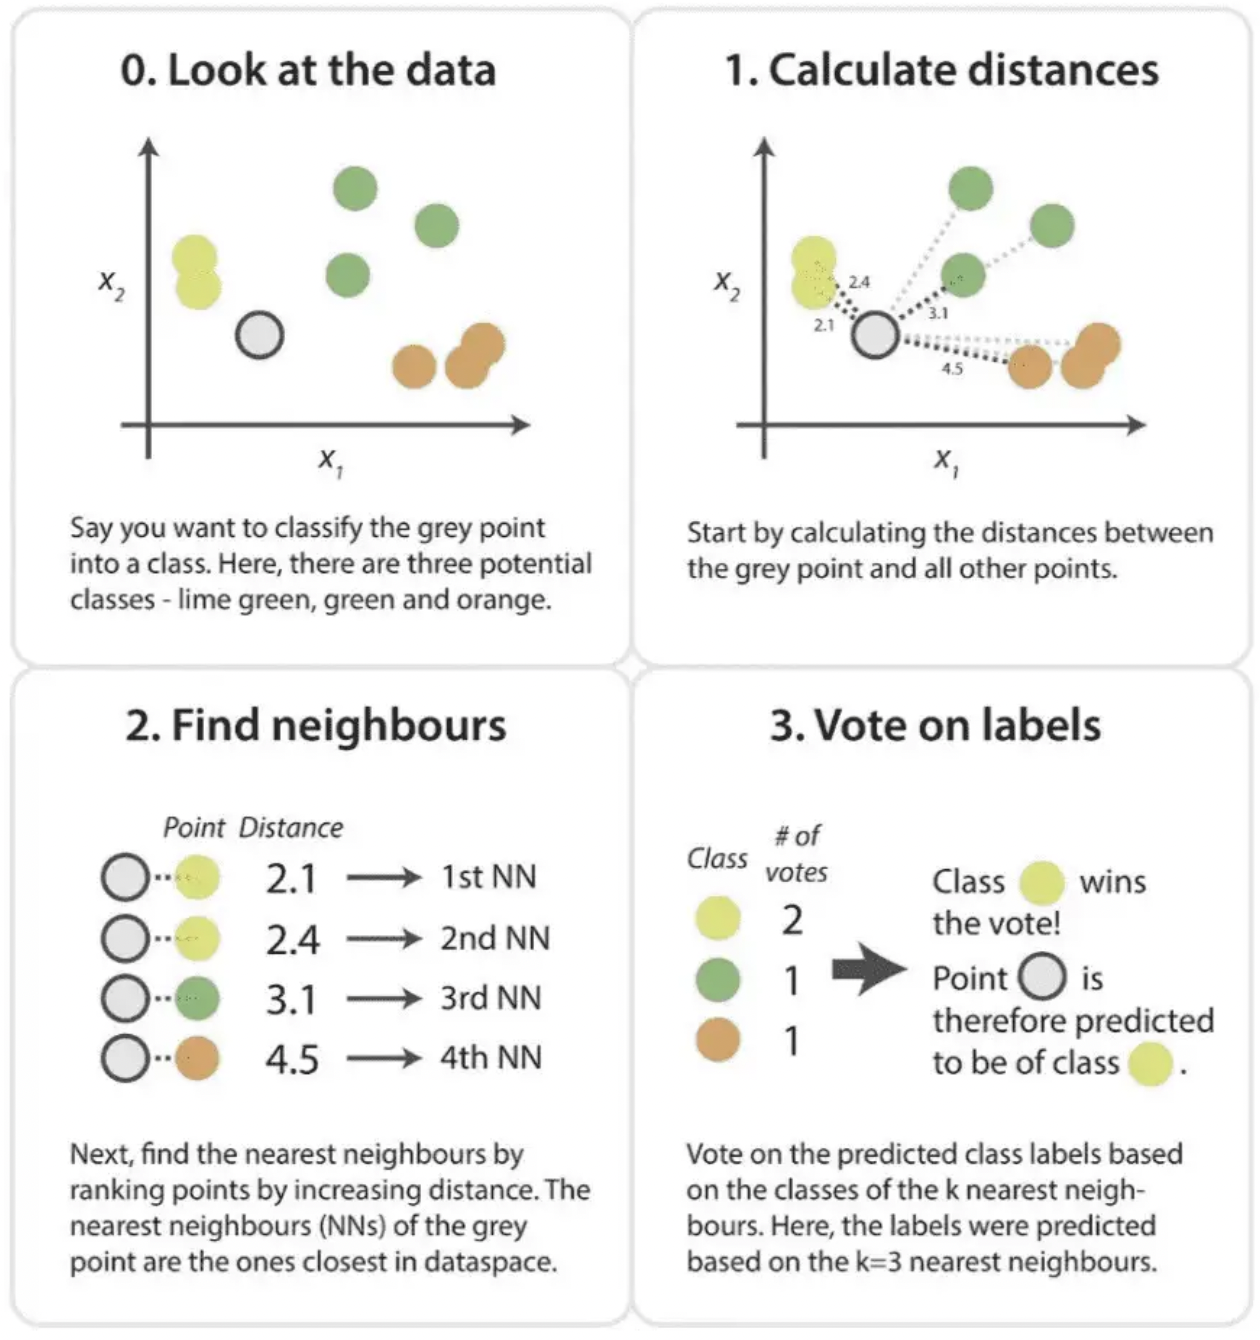
\includegraphics[scale=0.5]{images/knn/algo-main-phases.png}
    \caption{Explanation of the main phases of the KNN algorithm}
    \label{fig:knn_algorithm_main}
\end{figure}

Clearly, KNN is heavily reliant on the concept of distance between points, meaning mainly two things:

\begin{itemize}
    \item the choice of the measure of distance is heavily impactful on the behavior of the model; commonly used measures are variants of the \textit{Minkowski distance}, such as the \textit{Manhattan} or \textit{Euclidean} distances
    
    \item the model is sensitive to outliers and noise in the training data
\end{itemize}

At last, it is noted that, although it can be derived by using bayes theorem and the notion of density estimation, KNN is considered a discriminative classifier, mainly because its focus is predicting class labels instead of understanding the distribution of the features of a certain dataset. Hence, KNN is well suited to define decision boundaries to classify data, but not to generate it.

\subsection{The choice of K}

The image below shows that the algorithm behaves quite differently as the value of the hyperparameter $K$ changes.

\begin{figure}[h]
    \centering
    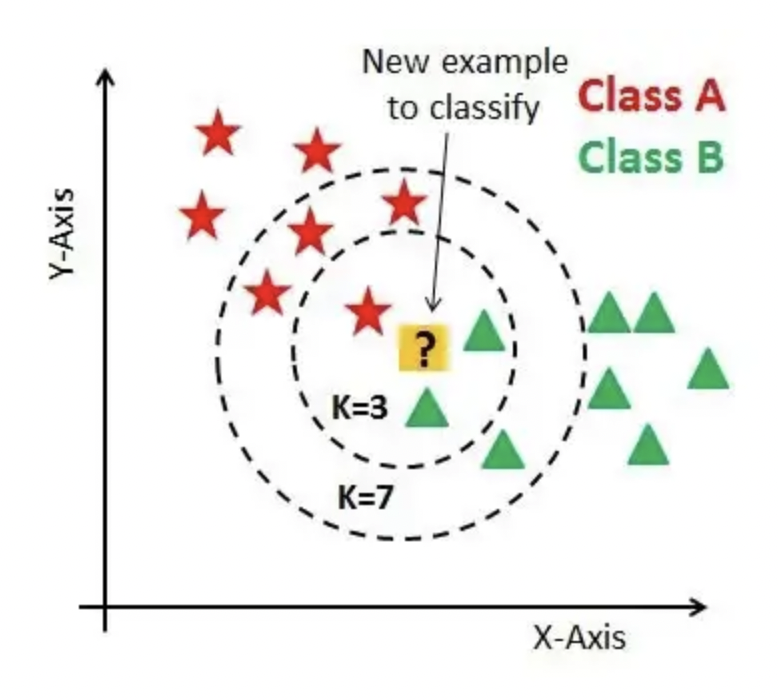
\includegraphics[scale=0.75]{images/knn/meaning-of-k.png}
    \caption{Visual representation of the impact of $K$ on the decision boundary}
    \label{fig:knn_k_hyperparam}
\end{figure}

Although there are no pre-defined formal methods to find the most favorable $K$, as a rule of thumb, small values of $K$ lead to unstable decision boundaries, with a behavior similar to overfitting, and as the value of $K$ approaches the total dimension of the training set, the precision of the model diminishes and asymptotically reaches the mean of the data.

\break
\section{Naive Bayes Classifier}

The Naive Bayes Classifier is a generative machine learning model that tries to estimate the probability distribution of the observations belonging to a certain class.

In order to understand the Naive Bayes approach, it is important to introduce Bayes’ Theorem. Bayes Theorem is a simple mathematical formula used for calculating conditional probabilities.

\begin{figure}[h]
    \centering
    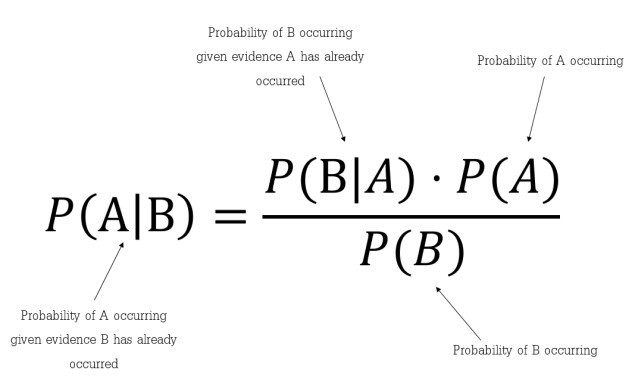
\includegraphics[scale=0.5]{images/naive-bayes/bayes-formula.jpg}
    \caption{Bayes Theorem statement with some comments}
    \label{fig:bayes_theorem_formula}
\end{figure}

Such a formula tells us how often $A$ happens given that $B$ happens, written $P[A \mid B]$ also called posterior probability, when we know:

\begin{itemize}
    \item how often B happens given that A happens, written $P[B \mid A]$
    \item how likely A is on its own, written $P[A]$
    \item how likely B is on its own, written $P[B]$
\end{itemize}


In order to align with the common terminology used for samples and class labels, we rewrite Bayes theorem as follows:

$$
\begin{aligned}
    P[Y = y \mid X = x] & = \frac{P[X = x \mid Y = y]P[Y = y]}{P[X = x]}
\end{aligned}
$$

where $x$ represents the sample that we want to make a prediction for, and $y$ represents the class that we want to calculate the probability for.
It is noted, however, that in a real world scenario, each 

The fundamental Naive Bayes assumption is that each feature makes an independent and equal contribution to the outcome. The assumptions made by Naive Bayes are generally not correct in real-world situations hence the name ‘Naive’. The independence assumption is never correct but often works well in practice.
Therefore, under the naive assumption, we can write:

$$
\begin{aligned}
    P[Y = y \mid X = (x_1, x_2, \dots, x_n)] & = \frac{P[X \mid Y = y]P[Y = y]}{P[X]} \\
    & = \frac{P[x_1 \mid y]P[x_2 \mid y] \dots P[x_n \mid y] P[y]}{P[x_1]P[x_2] \dots P[x_n]}
\end{aligned}
$$

where the vector $x = (x_1, x_2, \dots, x_n)$ represents the set of feature that the sample $x$ consists of. Note, in fact, that the conditional probability of each feature $x_i$ given class $y$ is taken independently of other features $x_j, j \ne i$.
Note that, if only full samples are considered, i.e. every feature is always taken into account, the denominator doesn't change, meaning that it can be removed to achieve proportionality as follows:

$$
P[y \mid x_1, \dots, x_n] \propto \prod_{i=1}^{n}{P[x_i \mid y]} P[y]
$$\label{theory_naive_bayes_formula}

Finally, predictions are obtained as follows:

$$
\begin{aligned}
    & P[Y = y \mid X = (x_1, x_2, \dots, x_n)] \\
    & \text{Find the most likely } y \to \text{prediction} = \text{argmax}_y P[Y = y \mid X = (x_1, x_2, \dots, x_n)] \\
\end{aligned}
$$


\break
\section{Training, Validation and Testing}

\subsection{Dataset Splits}

\begin{figure}[h]
    \centering
    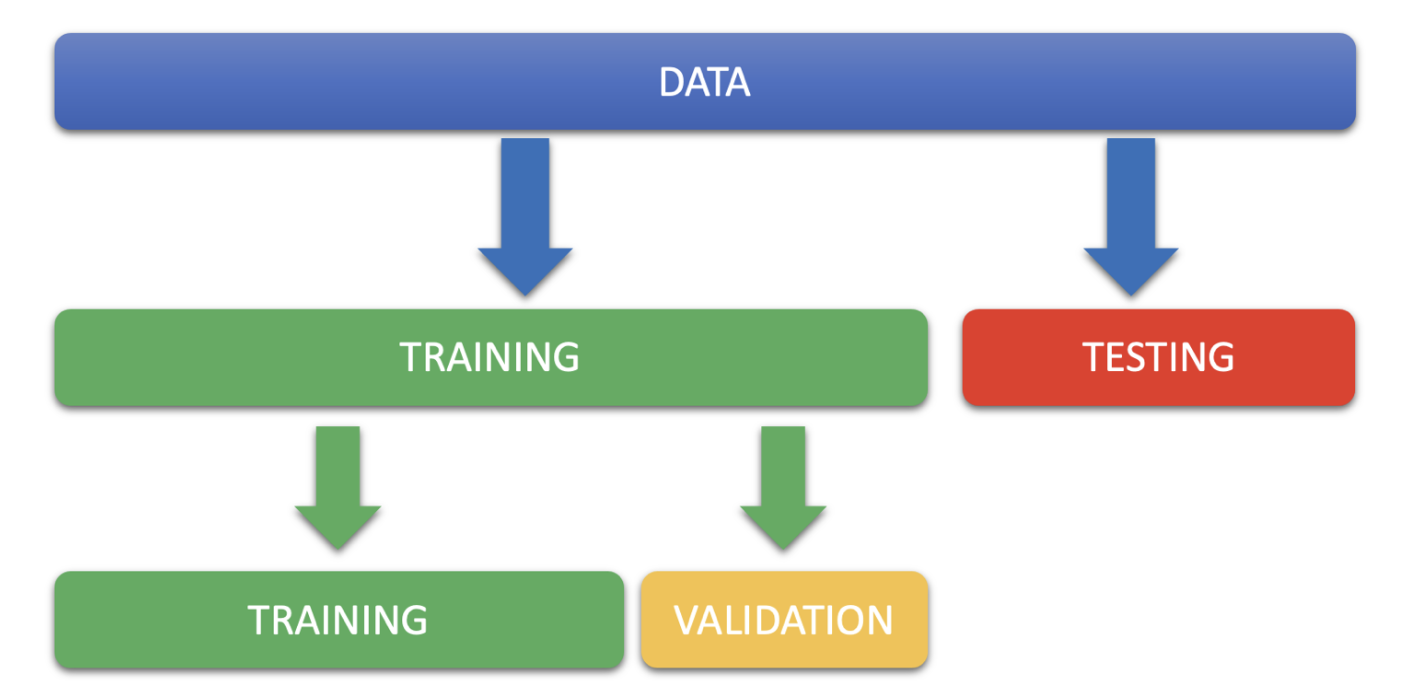
\includegraphics[scale=0.6]{images/train-val-test/train-val-test-split.png}
    \caption{Training, Validation, Testing splits of a dataset}
    \label{fig:train_val_test_splits}
\end{figure}

As it can be noted from the above image, a dataset used to train and tune a machine learning model must be divided in 3 parts:

\begin{itemize}
    \item \textbf{Training Set}, used to fit the model
    \item \textbf{Validation Set}, used to evaluate the model against different configurations of hyperparameters; it is sampled from the training set, usually in conjuction with the \textit{cross validation} technique, and can be thought of as a \textit{testing set for hyperparameters}
    \item \textbf{Testing Set}, used to evaluate the performance of the fully built model against new data
\end{itemize}

\subsection{K-Fold Cross Validation}

This technique is used in the validation phase, and its purpose is to avoid that the fraction of the training set that the validation set consists of is anomalous in some way, therefore negatively influencing the choice of hyperparameters for the model.
By performing the validation phase on $K$ combinations of training and validation sets, where each validation set does not overlap with the others, and then averaging the results obtained on each so called \textit{fold}, the tuning process becomes much more reliable. 
The following image summarises what previously mentioned:

\begin{figure}[h]
    \centering
    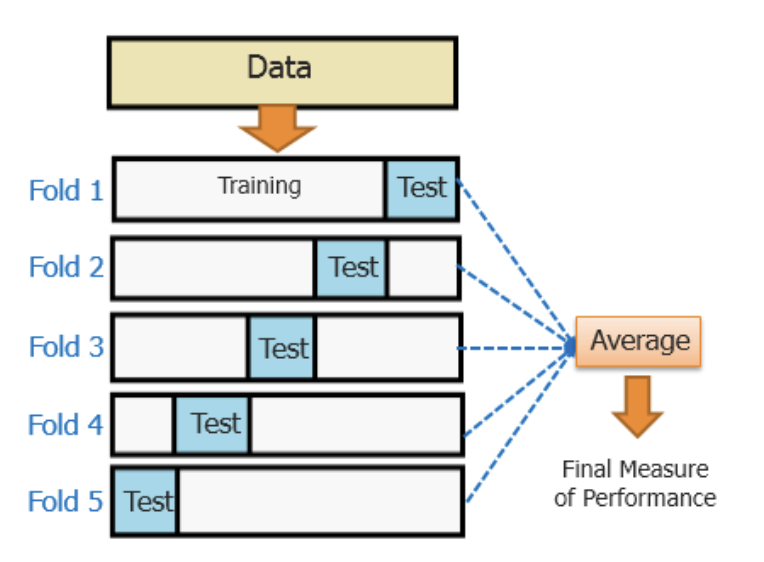
\includegraphics[scale=0.75]{images/train-val-test/cross-val.png}
    \caption{Visual representation of the k-fold cross validation technique}
    \label{fig:train_val_test_cross_val}
\end{figure}

\subsection{Grid Search With Cross Validation}

\textit{Grid search} is a tuning technique that attempts to compute the optimum values of hyperparameters. It is an exhaustive search that is performed on a specific set of hyperparameter values for some given model, that is, provided a set of values for each hyperparameter of the model, each combination of hyperparameters is evaluated against the validation set, and the best combination is kept. This technique is then combined with the previously discussed \textit{K-Fold Cross Validation} to more reliably choose the hyperparameters configuration.
The advantage of this technique is that, as aforementioned, a local optimum with respect to all the combinations of hyperparameters is found. This however, comes at the major disadvantage of poor scaling as the number of hyperparameters combinations increases, because of the big number of models to train and test.


\break
\section{Evaluation Metrics for Classifiers}

There is a plethora of evaluation metrics for classifiers, both binary and multiclass. For the purpose of this assignment, however, only 5 major ones will be discussed: \textbf{Accuracy}, \textbf{Precision}, \textbf{Recall}, \textbf{F1 Score} and \textbf{Confusion Matrix}

\paragraph{Accuracy} One of the more obvious metrics, it is the measure of all the correctly identified cases. It is most used when all the classes are equally important.

$$
Accuracy = \frac{
    \text{correctly predicted instances}}{
    \text{all predictions}}
$$

\paragraph{Precision (of class $y$)} It is implied as the measure of the correctly identified cases of $y$ from all the predicted $y$ cases. Thus, it is useful when the costs of misclassification is high.

$$
Precision_y = \frac{\text{correctly predicted as } y}{
    \text{correctly predicted as } y + \text{falsely predicted as } y
    }
$$

\paragraph{Recall (of class $y$)} It is the measure of the correctly identified $y$ cases from all the true $y$ cases. It is important when the cost of false negatives is high, i.e. when falsely predicting that some observation is not $y$, when it truly is, should be strongly avoided.

$$
Recall_y = \frac{\text{correctly predicted as } y}{
    \text{correctly predicted as } y + \text{falsely predicted as not } y
    }
$$

\paragraph{F1 Score} This is the harmonic mean of Precision and Recall and gives a better measure of the incorrectly classified cases than the Accuracy Metric.
Harmonic Mean is used since it more strongly penalizes extreme values when compared to the Arithmetic Mean.

$$
F1\ Score = 2 * \frac{Precision * Recall}{Precision + Recall}
$$

\paragraph{Confusion Matrix} A confusion matrix can give you a better idea of what your classification model is getting right and what types of errors it is making: accuracy alone can be misleading if you have an unequal number of observations in each class or if you have more than two classes in your dataset.
A confusion matrix is best explained through the below example image.

\begin{figure}[h]
    \centering
    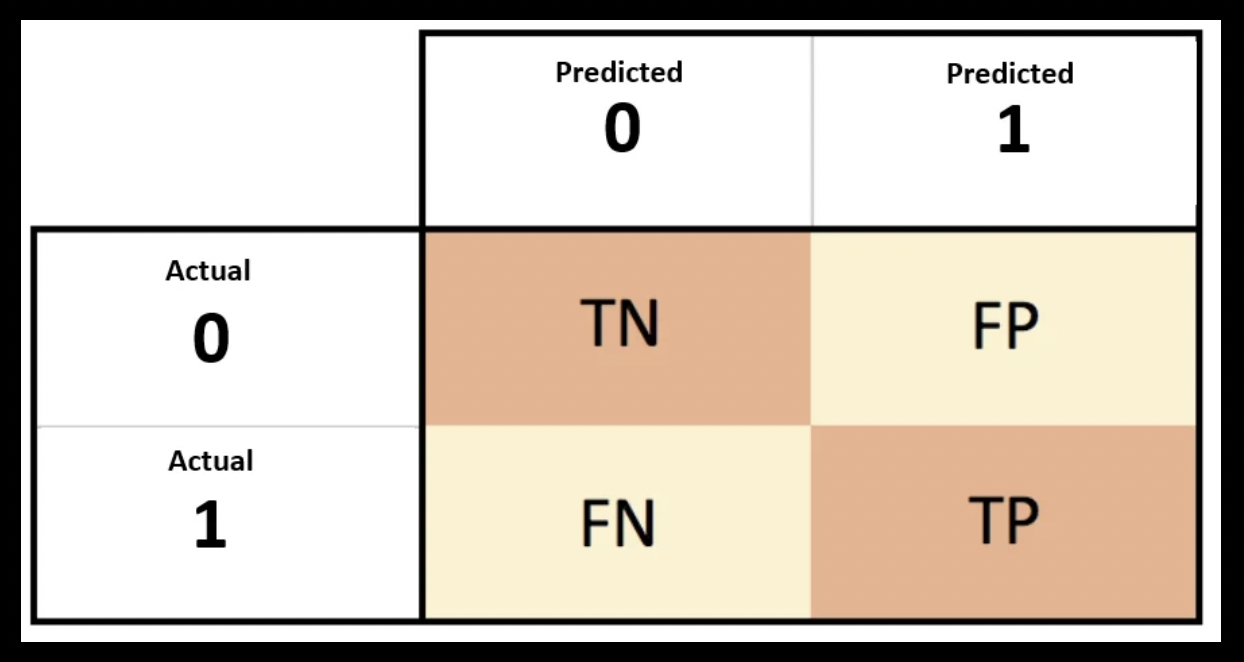
\includegraphics[scale=0.35]{images/eval-metrics/conf-matrix.png}
    \caption{Visual representation of confusion matrix; this example is for the binary classification case (just 2 classes), but in a multiclass scenario the same rules apply.}
    \label{fig:eval_metrics_conf_matrix}
\end{figure}


\paragraph{Rule of Thumb} Accuracy is used when the True Positives and True negatives are more important or when the dataset is balanced, while F1 Score is used when the cost of False Negatives and False Positives is high, or when the dataset is not balanced, meaning that some classes are much more or less probable than the others.
